% A21SequencesAndSeriesTikZ-002.tex
% Asset ID: A21SequencesAndSeriesTikZ-002
% Purpose: Geometric convergence and sum to infinity.
\documentclass[tikz,border=10pt]{standalone}
\usetikzlibrary{arrows.meta}
\begin{document}
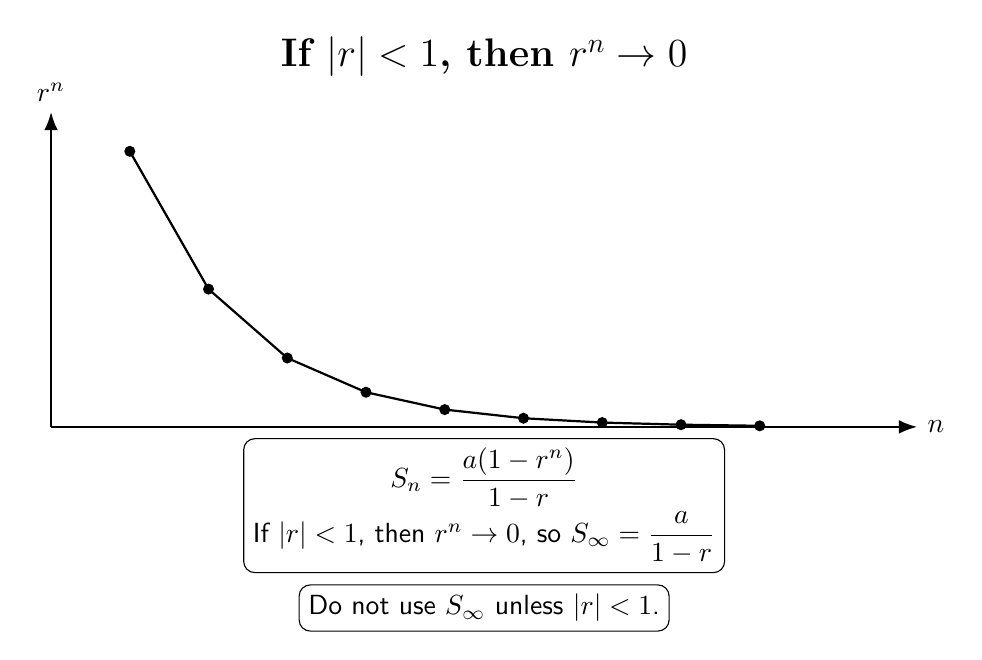
\begin{tikzpicture}[every node/.style={font=\sffamily}]
\node[font=\bfseries\Large] at (5.5,4.7){If $|r|<1$, then $r^n\to0$};
\draw[-{Latex},thick] (0,0)--(11,0) node[right]{$n$};
\draw[-{Latex},thick] (0,0)--(0,4) node[above]{$r^n$};
\draw[thick] plot coordinates {(1,3.5)(2,1.75)(3,0.875)(4,0.44)(5,0.22)(6,0.11)(7,0.055)(8,0.028)(9,0.014)};
\foreach \x/\y in {1/3.5,2/1.75,3/0.875,4/0.44,5/0.22,6/0.11,7/0.055,8/0.028,9/0.014}{\fill (\x,\y) circle (2pt);}
\node[draw,rounded corners,align=center] at (5.5,-1.0){$\displaystyle S_n=\frac{a(1-r^n)}{1-r}$\\If $|r|<1$, then $r^n\to0$, so $\displaystyle S_\infty=\frac{a}{1-r}$};
\node[draw,rounded corners] at (5.5,-2.3){Do not use $S_\infty$ unless $|r|<1$.};
\end{tikzpicture}
\end{document}
